\begin{frame}{Computing Correlation Functions in MPS}
\vskip-1.5cm
\only<1,3->{
\begin{figure}[t]
\centering
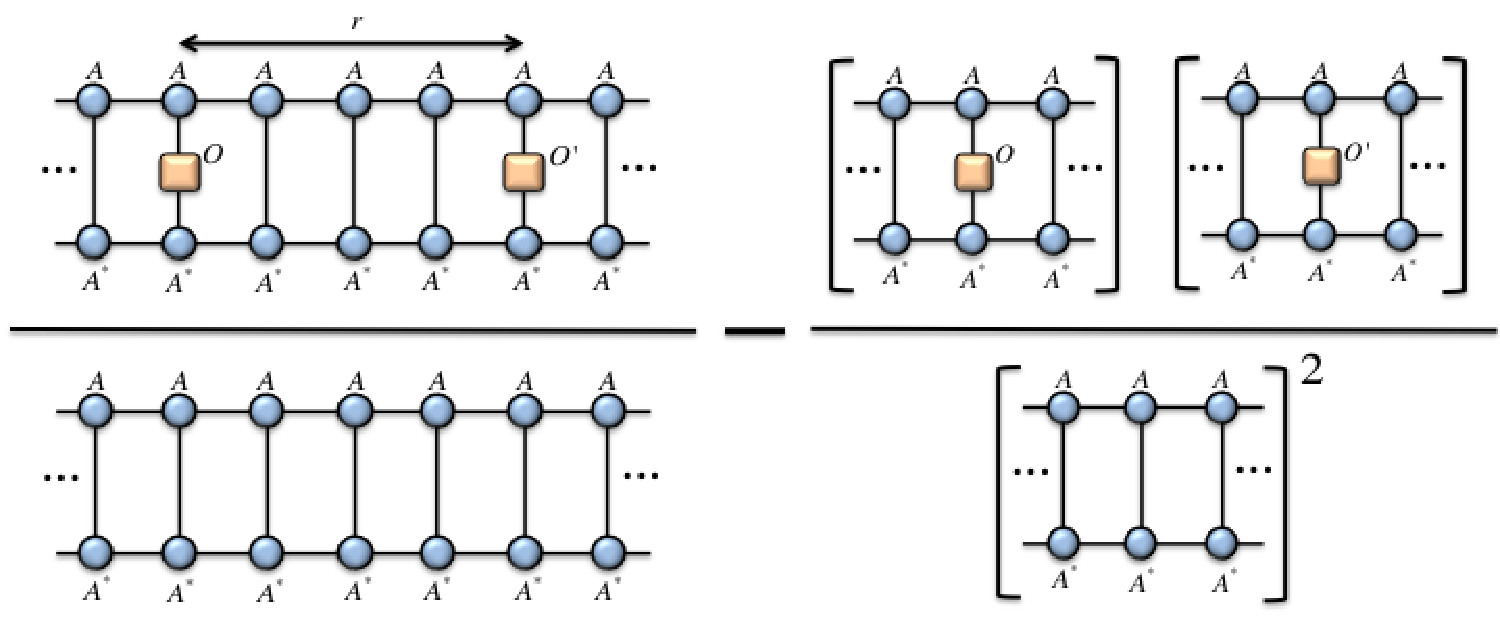
\includegraphics[width=\textwidth]{diagrams/orus-corrfunc.pdf}
%\begin{tikzpicture}[node distance=0.5cm]

\foreach \i in {1,...,5} {
	\node (Gp\i) at (1.5*\i,-2.5) [gamma] {};
	\node (Gpp\i) at ($ (Gp\i) + (0,-1) $) [gamma] {};
	\draw[thick] (Gp\i) -- (Gpp\i);
	\node[above of=Gp\i] {$A^\i$};
	\node[below of=Gpp\i] {$(A^\i)^*$};
}
\foreach \i / \j in {1/2,2/3,3/4,4/5} {
	\draw[thick] (Gp\i) -- (Gp\j);
	\draw[thick] (Gpp\i) -- (Gpp\j);
}

\foreach \i in {1,...,5} {
	\node (Gp\i) at (1.5*\i,-5.5) [gamma] {};
	\node (Gpp\i) at ($ (Gp\i) + (0,-2) $) [gamma] {};
	\node (O\i) at ($ (Gp\i) + (-0,-1) $) [operator] {};
	
	\draw[thick] (Gp\i) -- (O\i);
	\draw[thick] (Gpp\i) -- (O\i);
	
	\node[above of=Gp\i] {$A^\i$};
	\node[below of=Gpp\i] {$(A^\i)^*$};
	\node[above left of=O\i] {$W^\i$};
}
\foreach \i / \j in {1/2,2/3,3/4,4/5} {
	\draw[thick] (Gp\i) -- (Gp\j);
	\draw[thick] (Gpp\i) -- (Gpp\j);
	\draw[thick] (O\i) -- (O\j);
}

\end{tikzpicture}

\caption{Diagram for $C_{O O'}(r) = \ev{O_i O'_{i+r}}- \ev{O_i}\ev{O'_{i+r}}$}
\end{figure}
}
\only<2>{
\begin{columns}[T]
    \begin{column}[T]{.28\textwidth}
        \begin{figure}[h]
            \centering
            \scalebox{1}{
            \begin{tikzpicture}[node distance=0.4cm]
\begin{scope}[thick, decoration={
    markings,
    mark=at position 0.5 with {\arrow{>}}}
    ]
  \node[gamma] (A) at (0,0) {$A$};  
  \node[gamma] (Ac) at (0,2) {$A^{*}$};
  \draw[postaction={decorate}] (A)--(Ac);
  \node[inv] (ki) at (1, 0){};
  \node[inv] (bi) at (1, 2){}; 
  \node[inv] (ko) at (-1, 0){}; 
  \node[inv] (bo) at (-1, 2){};
  \draw[color=red, postaction={decorate}] (ki)--(A);
  \draw[color=green, postaction={decorate}] (bi)--(Ac);
  \draw[color=red, postaction={decorate}] (A) -- (ko);
  \draw[color=green, postaction={decorate}] (Ac) -- (bo);

\end{scope}
\end{tikzpicture}

            }
            \caption{Transfer Matrix $\mathbb{E}_{I}$}
            \note{Reminder using arrows to represent in and out}
        \end{figure}
    \end{column}
    \begin{column}[T]{.3\textwidth}
        \begin{figure}[h]
            \centering
            \scalebox{1}{
            \begin{tikzpicture}[node distance=0.4cm]
\begin{scope}[thick, decoration={
    markings,
    mark=at position 0.5 with {\arrow{>}}}
    ]
  \node[gamma] (A) at (0,0) {$A$};  
  \node[operator] (O) at (0, 1) {$O$};
 % \node[operator] (O2) at (0, 1) {$O'$};
  \node[gamma] (Ac) at (0,2) {$A^{*}$};
  \draw[postaction={decorate}] (A)-- (O) -- (Ac);
  \node[inv] (ki) at (1, 0){};
  \node[inv] (bi) at (1, 2){}; 
  \node[inv] (ko) at (-1, 0){}; 
  \node[inv] (bo) at (-1, 2){};
  \draw[color=red, postaction={decorate}] (ki)--(A);
  \draw[color=green, postaction={decorate}] (bi)--(Ac);
  \draw[color=red, postaction={decorate}] (A) -- (ko);
  \draw[color=green, postaction={decorate}] (Ac) -- (bo);

\end{scope}
\end{tikzpicture}
            }
            \caption{Operator Insertion $\mathbb{E}_{O}$}
        \end{figure}
    \end{column}
    \begin{column}[T]{.42\textwidth}
        \vskip1.8cm
        \begin{figure}[h]
            \centering
            \scalebox{0.8}{
            \begin{tikzpicture}
\begin{scope}[very thick,decoration={
    markings,
    mark=at position 0.5 with {\arrow{>}}}
    ] 

\node[peps] (A1) at (-4.1, 0) {};
\node (li) at ($(A1) + (-1, 0) $) {};
\draw[thick, postaction={decorate}] (li.center) -- (A1.west);
\draw[thick, postaction={decorate}] (A1.east) -- node[right] {} +(1,0);
\draw[thick, postaction={decorate}] (A1.north) -- node[above] {} +(0,0.5);

\node at (-2.3, 0.5){$= e^{i \theta}$};    

\node[peps] (A) at (0, 0) {};
\node[draw] (Ul) at ($(A) + (-1, 0) $) {$U$};
\node[draw] (Ur) at ($(A) + (1, 0) $) {$U^{\dagger}$};
\node (LI) at ($(Ul) + (-1, 0) $) {};
\draw[thick, postaction={decorate}] (LI.center) -- (Ul.west);
\draw[thick, postaction={decorate}] (Ur.east) -- node[right] {} +(0.5,0);
\draw[thick, postaction={decorate}] (Ul) -- (A);
\draw[thick, postaction={decorate}] (A) -- (Ur);
\draw[thick, postaction={decorate}] (A.north) -- node[above] {} +(0,0.5);

\end{scope}
\end{tikzpicture}
            }
            \caption{MPS gauge redundancy}
        \end{figure}
    \end{column}
\end{columns} 
\begin{figure}[h]
    \centering
    \scalebox{1}{
    \begin{tikzpicture}[node distance=0.4cm]
\begin{scope}[thick, decoration={
    markings,
    mark=at position 0.5 with {\arrow{>}}}
    ]
  \node[gamma] (A) at (0,0) {$A$};  
  \node[gamma] (Ac) at (0,2) {$A^{*}$};
  \node[side, minimum height=1.97cm] (vR) at (1.5, 1){$v_R$};
  \draw[postaction={decorate}] (A)--(Ac);
  \node[inv] (ki) at (1, 0){};
  \node[inv] (bi) at (1, 2){}; 
  \node[inv] (ko) at (-1, 0){}; 
  \node[inv] (bo) at (-1, 2){};
  \draw[color=red, postaction={decorate}] (vR.south west) -- (ki.center)--(A);
  \draw[color=green, postaction={decorate}] (vR.north west)-- (bi.center)--(Ac);
  \draw[color=red, postaction={decorate}] (A) -- (ko);
  \draw[color=green, postaction={decorate}] (Ac) -- (bo);
  
  \node[] at (2.5, 1){$=$};
  \node[side, minimum height=1.97cm] (vR) at (3.5, 1){$v_R$};
  \node[inv] (ki) at (2.5, 0){};
  \node[inv] (bi) at (2.5, 2){};
  \draw[color=red, postaction={decorate}] (vR.south west) -- (ki.center);
  \draw[color=green, postaction={decorate}] (vR.north west)-- (bi.center); 

  \node[] at (4.5, 1){$=$};
  \node[side, minimum height=0.6cm] (sR) at (5.5, 0){$\sigma_R$};
  \node[inv] (ki) at (4.5, 0){};
  \node[inv] (k2) at (6.3, 0){};
  \node[cdot] (dot) at (6.3, 1){};
   \node[inv] (b2) at (6.3, 2){};
  \node[inv] (bi) at (4.5, 2){};
  \draw[color=red, postaction={decorate}]  (dot)--(k2.center);
  \draw[color=red, postaction={decorate}]  (k2.center)-- (sR.east);
  \draw[color=red, postaction={decorate}]  (sR.west) -- (ki.center);
  \draw[color=green, postaction={decorate}]  (dot)--(b2.center);
  \draw[color=green, postaction={decorate}]  (b2.center)-- (bi);
\end{scope}
\end{tikzpicture}
    }
\caption{Eigenvector equation $\mathbb{E}_{I}(\sigma_R) = \sigma_R$}
\end{figure}
   
}
\only<3>{
\vskip-0.5cm
 $$\ev{O_i O'_{i+r}} = \vbraopket{v_L}{\mathbb{E}_O \mathbb{E}_I^r \mathbb{E}_{O'}}{v_R}$$
 $$
 \lim\limits_{r \rightarrow \infty} \ev{O_i O'_{i+r}} = \vbraopket{v_L}{\mathbb{E}_O}{v_R} \vbraopket{v_L}{\mathbb{E}_{O'}}{v_R}
 $$
 $$ C_{O O'}(r) \approx const. \times \lambda_2^r $$
\note{Matrix product states also known as finitely correlated states}
}
\end{frame}